\subsection{How one detects vehicles violating the speed limit when
all one has is a stationary camera}

\noindent Context: EL2320 Applied Estimation Project\\
\noindent KTH Royal Institute of Technology, Stockholm, Sweden; 2016\\

\noindent \href{https://github.com/li9i/HT15_P2_EL2320_Lab_1}{\texttt{[Kalman filter \ \ implementation and documentation]}}

 \noindent \href{https://github.com/li9i/HT15_P2_EL2320_Lab_2}{\texttt{[Particle filter implementation and documentation]}}\\


\begin{problem}
Assume a stationary camera overseeing a stretch of road on
which vehicles travel freely. We would like to identify vehicles travelling at
a speed larger than a given threshold.
\end{problem}

One solution is comprised of two segments: (a) At first, a differentiation
between what is considered background (the unvaried and vehicle-less road scene)
and what is considered foreground (the objects ``travelling" on top of the
background) is in order. Since the data is in video form, we need to track
the colour of each pixel through time, and therefore perform segmentation via
Gaussian Mixture Models. (b) After vehicles have been detected, a separate
Kalman filter (alternatively, a Particle filter) estimates the vector of the
velocity of each detected vehicle. Given that the camera is stationary,
information (or even guesstimates) about its placement with respect to the
road it oversees can establish a correspondence between a vehicle's real (road)
velocity and represented (image) velocity, so that vehicles above the speed
limit are identified. Image \ref{fig:kf_1} shows a frame drawn from a video
sequence where the position and velocity of two vehicles are being tracked.

\begin{figure}[H]\centering
  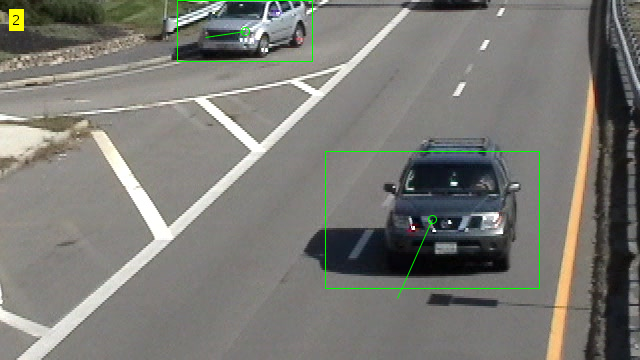
\includegraphics[scale=0.55]{images/kf_1.png}
  \caption{\small Two vehicles are successfully detected, with their velocity
           vector being estimated through time, using one Kalman filter per
           vehicle}
  \label{fig:kf_1}
\end{figure}

\begin{itemize}
\item Notions/resources/tools used: video segmentation, Gaussian Mixture Models, Kalman filter,
Particle filter, MATLAB
\end{itemize}
